\documentclass[a4paper, 10pt]{article}
\usepackage[margin=1in]{geometry} 
\usepackage{amsmath}
\usepackage{tcolorbox}
\usepackage{amssymb}
\usepackage{amsthm}
\usepackage{lastpage}
\usepackage{fancyhdr}
\usepackage{accents}
\usepackage{titlesec}
\usepackage{graphicx}
\usepackage{hyperref}

\usepackage{titling}
\usepackage[export]{adjustbox}

\usepackage{enumitem}
\setlist{nolistsep}

\usepackage[scaled]{helvet}
\renewcommand\familydefault{\sfdefault} 
\usepackage[T1]{fontenc}
\usepackage{tcolorbox}
\definecolor{light-blue}{cmyk}{0.24, 0.12, 0.0, 0.04, 1.00}

\setlength{\parindent}{0pt}
\setlength{\parskip}{6pt}%

%parskip shold take care of heading spacing
\titlespacing\section{0pt}{0pt}{0pt}
\titlespacing\subsection{0pt}{0pt}{0pt}
\titlespacing\subsubsection{0pt}{0pt}{0pt}


\pagestyle{fancy}
\setlength{\headheight}{40pt}

\hypersetup{
    colorlinks=true,
    linkcolor=blue,
    filecolor=magenta,      
    urlcolor=black,
    pdfpagemode=FullScreen,
}

\begin{document}

%REPLACE THE TEXT BELOW WITH YOUR NAME, STUDENT NUMBER AND ASSIGNMENT NUMBER
\lhead{Alexander Sepelenco (20335014)} 
\rhead{CS7GV6 – Computer Graphics Deliverable 1} 
\cfoot{\thepage\ of \pageref{LastPage}}

\begin{tcolorbox}[colback=light-blue]
\begin{small}
\textbf{DECLARATION:} I understand that this is an \textbf{individual} assessment and that collaboration is not permitted. I have read, understand and agree to abide by the plagiarism provisions in the
General Regulations of the University Calendar for the
current year, found at http://www.tcd.ie/calendar.
I understand that by returning this declaration with my work, I am agreeing with the above statement. 
\end{small}
\end{tcolorbox}

\bigskip
%OPTIONAL: INSERT A TITLE BY UN-COMMENTING THE NEXT LINE
%\Large\textbf{Project Proposal and Design Document} \normalsize

%15/10/2022: Deliverable 1 - Project Proposal and Design Document (5 Marks)
%    Submit a written proposal (1-2 pages) outlining your intended underwater ecosystem
%    Describe key features you plan to implement (types of marine life, lighting effects, unique interactions)
%    Mention any advanced or custom features that you are considering
%    Include sketches, diagrams or screenshot illustrating the scene layout


\section{Project Proposal and Design Document}
I selected the project "Manta Ray Migration – Simulate a large school of manta rays gliding through a dynamic ocean, interacting with smaller fish".
And the theme is called "Dynamic Underwater Ecosystem Simulation". It is important to define my project and the broad theme to scope out the work involved.

\subsection{Advanced/Custom features I am considering}
\begin{itemize}
    \item Boids (for simulating marine life)
    \item Fog (for water)
    \item Sky box
    \item Fluid animation using lerp (linear interpolating between positions)
    \item Using Quaternion for rotations to avoid gimble lock
    \item Instancing draw calls
\end{itemize}

One feature that I am considering for my project is intelligent character behavior. Specifically I am considering Boids \cite{boids} by Craig Reynolds, for my interaction 
between my manta rays and small fish. I think this advanced feature is important to make an interesting simulation. I am also considering Boids for my crabs and starfish,
where the starfish are obstacles for the crabs, which would make for interesting simulation of walking. 
For water effects, I want to implement a blue fog, simulating water of an ocean. I think adding a skybox would make the scene more realistic as well. I will also use quaternions for rotating my marine life,
before they hit each other, to make it realistic. I will use lerp to linearly interpolate between the point of rotation and the previous point to add fluidity to the movement. My final advanced feature would
be to instance drawing multiple of the same models, so that we can optimize and reduce the amount of draw calls required to draw my marine life. Specifically I will instance my marine life like manta rays.

\subsection{Outlining my types of marine life}
\begin{itemize}
    \item Manta Ray
    \item Small Fish
    \item Starfish
    \item Crab
\end{itemize}
Specifically, I'm thinking of adding hierarchical animation for my small fish and my crabs. Although I may decide to have another underwater createure, because animating 10 legs on a crab
might be more hassle than its worth. I think a manta ray flapping animation based on hierarchical structure could work well. What I mean by this is splitting the left and right side of the 
fins of the mantaray and using hierarchical structure moving each section of the fin. The sketch below hopefully describes what I mean

\begin{figure}[h!]
    \centering
    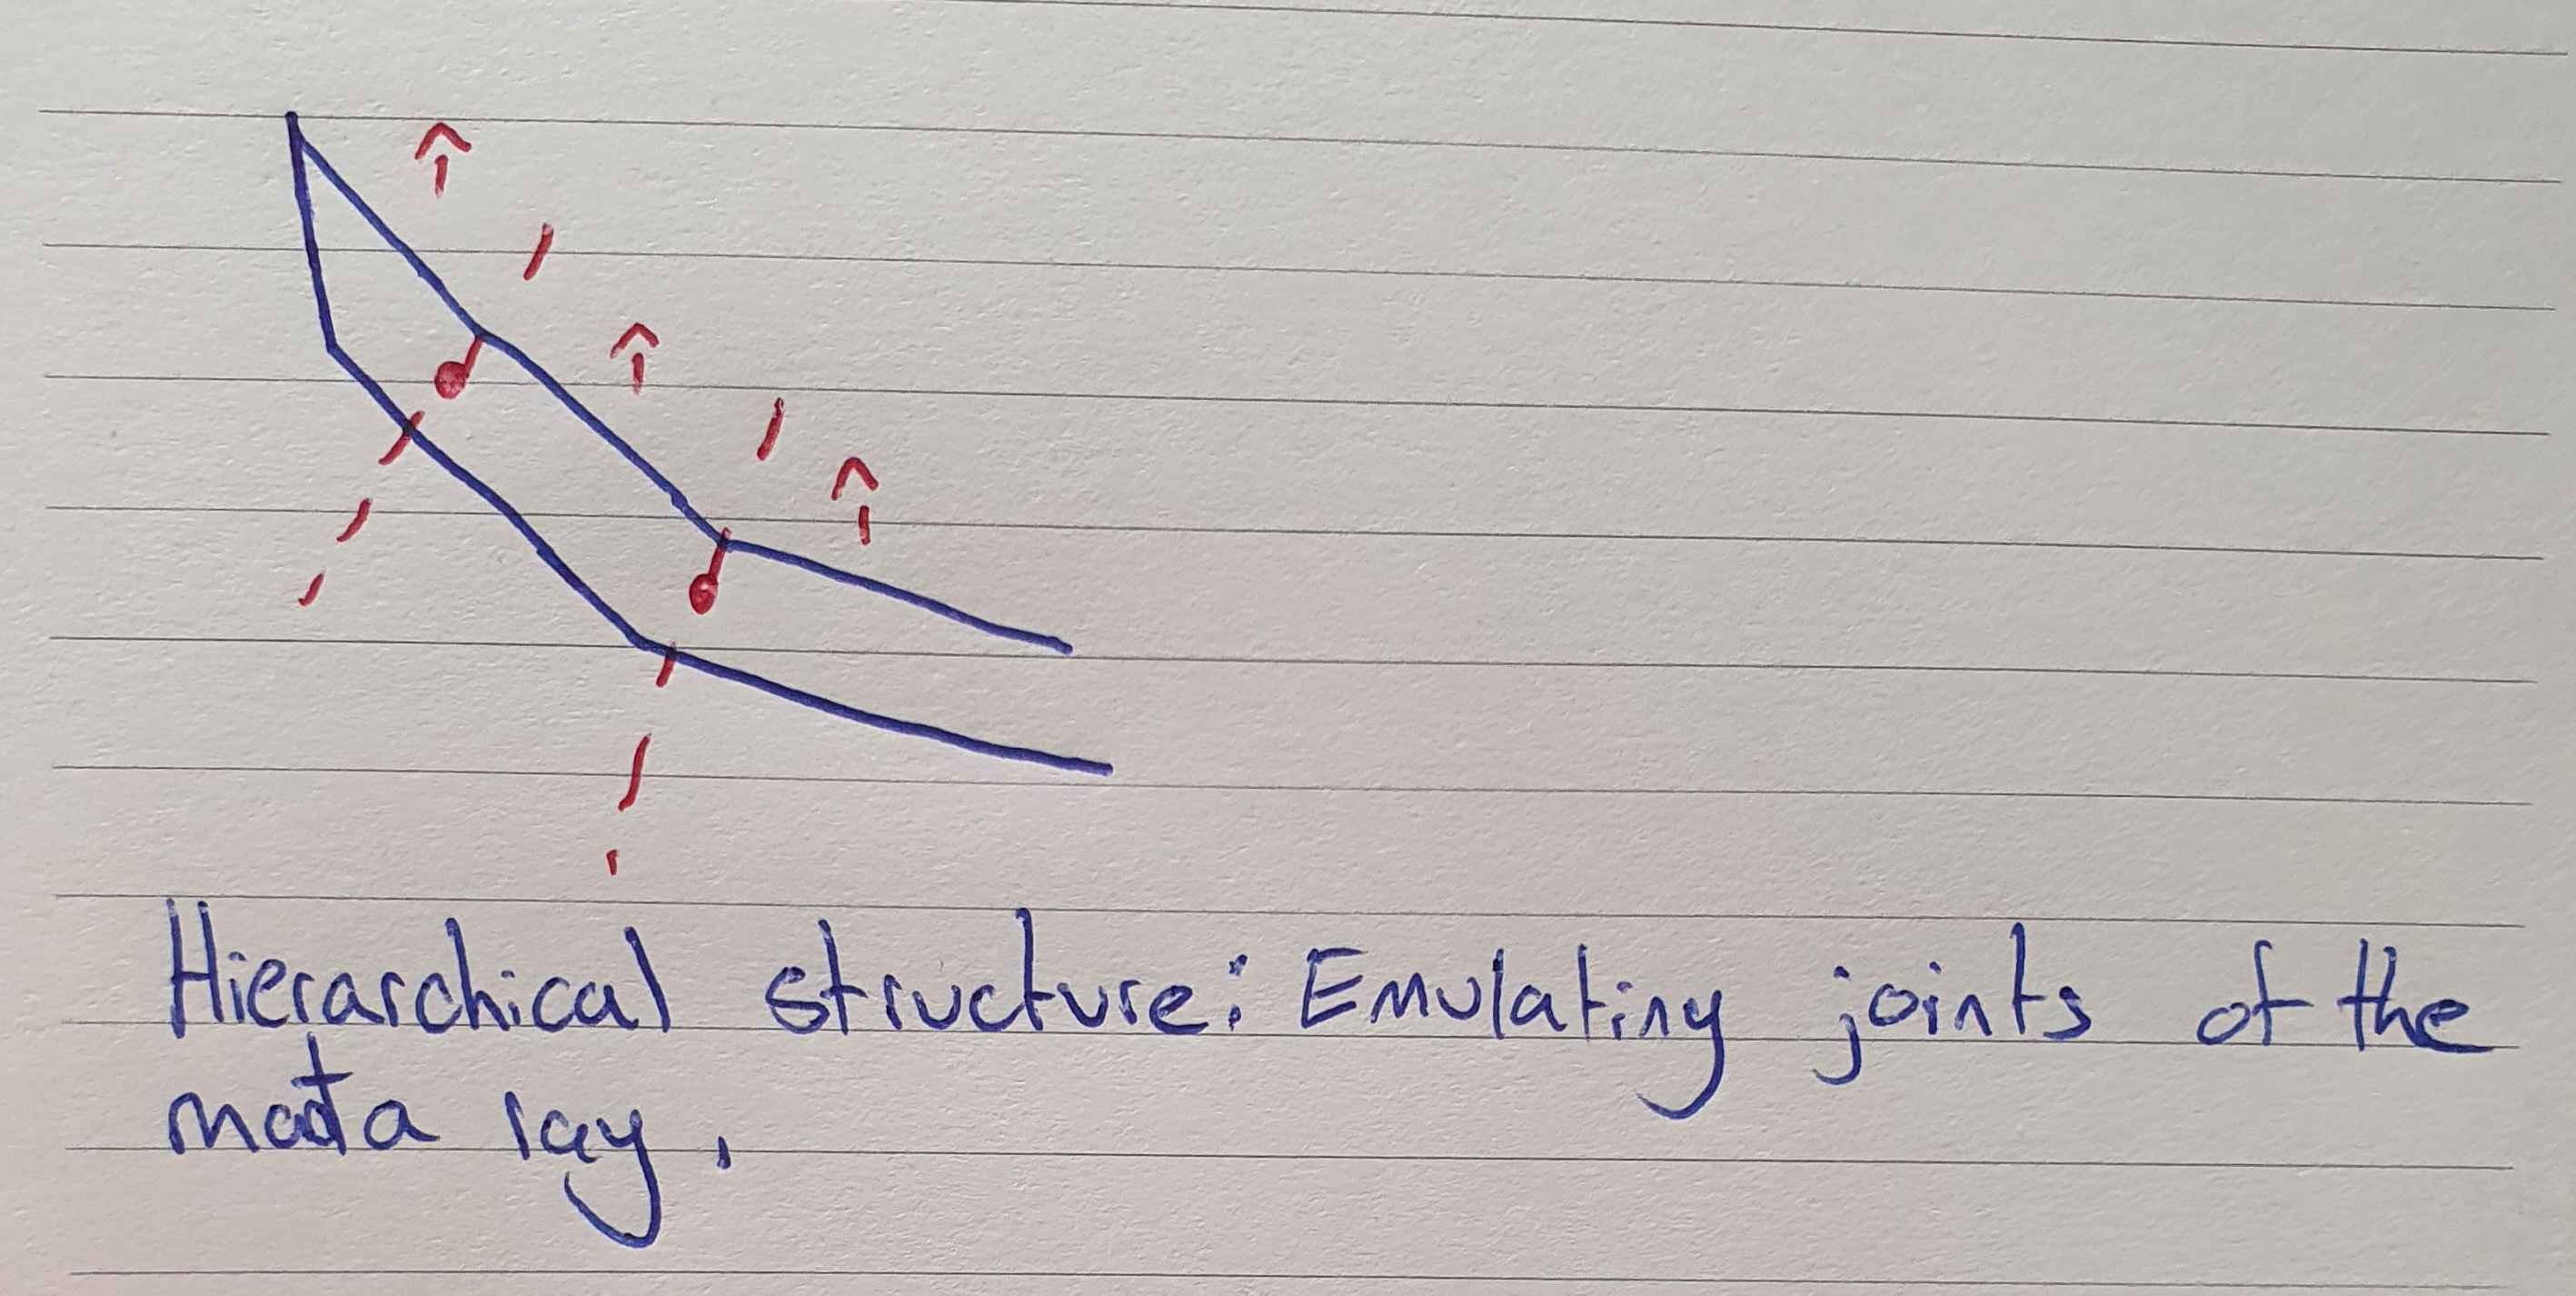
\includegraphics[scale=0.1]{images/mantaray-sketch.jpg}
    \caption{Sketch of the manta ray hierarchical structure}
    \label{fig:mantaray-sketch}
\end{figure}

\begin{figure}[h!]
    \centering
    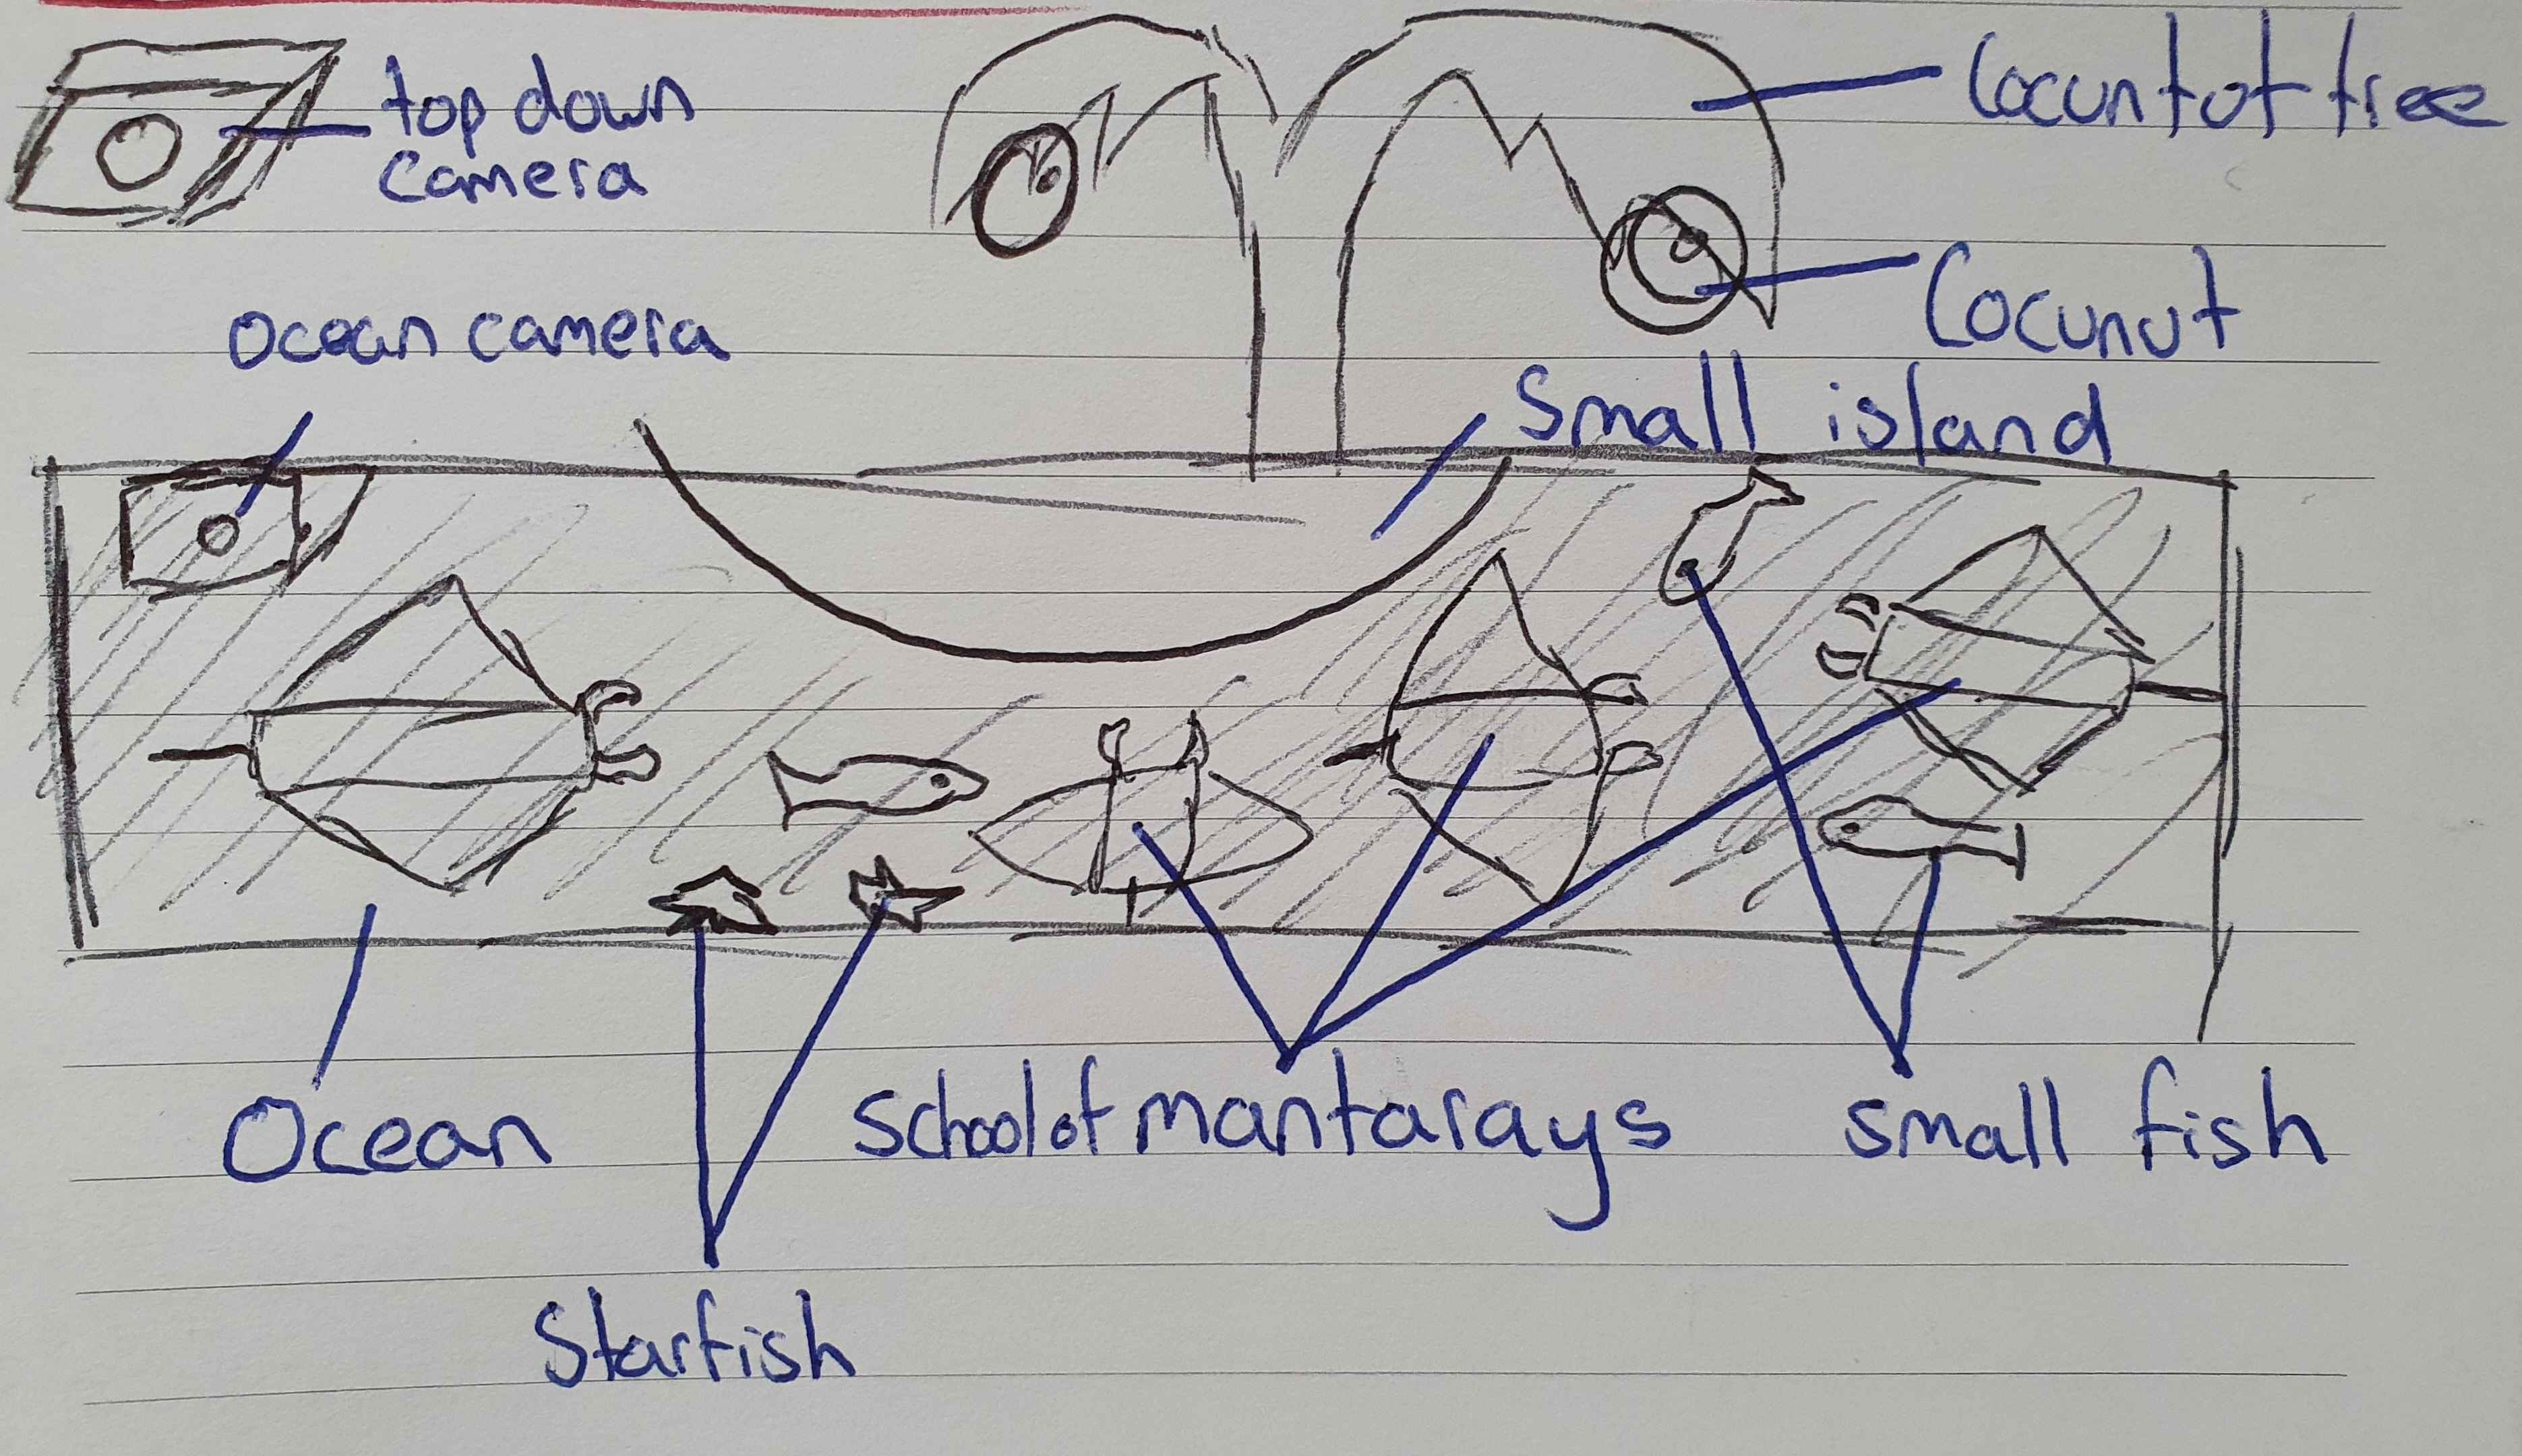
\includegraphics[scale=0.1]{images/sketch.jpg}
    \caption{Sketch of the environment}
    \label{fig:environment}
\end{figure}

\newpage

\subsection{Outlining my types of non marine life}
\begin{itemize}
    \item Coconut + Coconut tree
    \item Underwater seaweed (potentially bioluminescent)
    \item grass
    \item sand
\end{itemize}

I want my non marine life to complement my theme, and project. I want some patch of land on my ocean, so that I can demonstrate alpha blending of transparent grass. My underwater seaweed
will be bioluminescent, meaning it will cast a light on my marine life. The light will be a Phong illumination light, with point lights in the seaweed, and a general direction light above
my landscape as the direction of a sun/daylight. I want a coconut on my patch of sand as well to add some personality to the environment.

% feel free to use bibtex
\begin{thebibliography}{9}
\bibitem{boids}
Boids: Artifical life Simulation
\textit{https://en.wikipedia.org/wiki/Craig\_Reynolds\_(computer\_graphics)}
\textit{Craig Reynolds}
\end{thebibliography}


\end{document}


